\documentclass[12pt]{article}
\usepackage[utf8]{inputenc}
\usepackage[ruled,vlined]{algorithm2e}
\usepackage[colorlinks]{hyperref}
\usepackage{capt-of}
\usepackage{amssymb}
\usepackage{amsmath}
\usepackage{url}
\usepackage{graphicx}
\usepackage{color}
\usepackage{bbm}
\usepackage{float}
\usepackage{listings}
\usepackage{subcaption}
\usepackage{setspace}
\onehalfspacing
\usepackage{geometry}


\title{Customized Hybrid Convolutional Layers in Deep Learning Models}
\author{Genglin Liu, Ina Fiterau }
\date{May 2021}

\begin{document}

\maketitle

\section{Abstract}
Deep learning has been widely used in computer vision tasks in recent years, due to the strong approximation capability of deep neural networks and more specifically, the feature extraction capability of convolutional neural networks. Deep learning models are proven to be very strong in extracting features from unstructured data such as images, text or temporal signals. However, at times there is also a rich amount of structured information such as demographic information of patient records along with medical images, which may contribute to the tasks at interest. Most current deep learning models do not jointly optimize over the images along with any structured covariates even if they are available. We propose a hybrid deep learning mechanism that takes available structured information into account during the feature extraction process, and consequently boosts the accuracy for certain classification tasks. Compared against our baseline models, hybrid counterparts perform 2\%-3\% better on the CelebA facial attribute dataset, and we hope to extend this technique to medical neuroimaging analysis and aid tasks such as early Alzheimer's detection.


\section{Introduction}

The main problem we're investigating in this thesis is the binary prediction of a facial attribute in the CelebA dataset using deep learning. We explore whether the hybrid convolution that involves structured covariates could yield in better performance than a neural network with regular convolutional layers. Although most of our work so far is done with human face images, we suggest that this mechanism will have more useful impact on tasks concerning biomedical data such as medical scans with patient records or domain-specific medical exam evaluations. The rest of this paper will present our effort of building the hybrid convolutional layer, modifying our baseline architecture and fusing multiple covariates into our feature extraction, and tuning the relevant hyperparameters to refine the performance of the novel network.

\subsection{VGG}
we selected the VGG Net [reference] as the baseline model for my experiments. There were a few other popular options to choose from, such as Residual network (ResNet) [reference] or an older network such as AlexNet [reference], but VGG turned out to be the ideal candidate. The reason is that VGG has a very straightforward architecture compared to ResNet which has more complex skip connections between layers. As we start building a new model, it is more reasonable to start with simpler architectures. On the other hand, AlexNet, along with many other older and simpler architectures, are not powerful enough to reach the level of performance that VGG does on image recognition tasks. 

The VGG neural network architecture used in our experiments is the VGG-16 architecture. This architecture consists of total 16 layers which is divided into a `feature extractor' container of 13 convolutional layers, 2 hidden fully connected layer, and 1 fully connected output layer. Every convolutional layer and
the fully connected hidden layer is followed by Rectified Linear Unit (ReLU) nonlinear function. The output layer has 2 output neurons followed by a Softmax layer to produce probability outputs.

\subsection{CelebA dataset}

We experiment our hybrid convolutional layers on a toy dataset before we move on to the ADNI data and apply it to the MRI image feature extractors.

We use the CelebFaces dataset[reference] which contains 202,599 face
images of 10,177 identities (celebrities) collected from
the internet and annotated with 40 facial attributes. The dataset is split into 162,770 instances for training and 19,962 instances for testing. For our purposes we test on the validation set which contains 19,867 instances, each time after we train our models on the entire training set. 

The toy problem we are solving in this section is to predict a binary facial attribute in the CelebA dataset using a deep convolutional network VGG Net. Later we will investigate whether the shortfused hybrid convolutional layers improve performance on the same classification task.

\subsection{Significance and Relevance to Neuroimaging and Alzheimer's Detection}

Alzheimer’s disease (AD)  is a degenerative condition that causes major changes in the brain, leading to cognitive decline and death in a matter of a few years. There is no known effective cure for the Alzheimer's. Many treatments have been tried, immense effort has been expended into clinical trials and nothing has worked so far. The main reason is that, usually by the time Alzheimer's is diagnosed, 60\% of brain matter is gone and the process is irreversible.

Most of the existing clinical trials fail to help identify a cure to the disease and a lot of pharmaceutical companies have invested and an estimated 150 to 300 experimental Alzheimer's treatments have failed to show clinical benefits. 

As an open challenge in healthcare, diagnosing and forecasting the Alzheimer's Disease have been studied a lot by healthcare professionals and data scientists. Current popular forecasting models tend to use hand-crafted volumetric features from brain magnetic resonance imaging (MRI) as input, which may not be as informative as features extracted directly from the scans themselves. 

We propose a novel forecasting framework which takes patient MRI scans as input and utilizes a deep 3D Convolutional Neural Network (CNN) to extract features from a patient’s brain MRIs over multiple visits. We then fuse these features extracted from the neural network with the cognitive test scores of a patient and demographic data. These features are then fed into a Recurrent Neural Network, which can provide an insight into the patient’s disease progression over time. We show that the inclusion of these customised/patient-specific features increases the F1-score, sensitivity, and specificity of forecasting the disease stage of cognitively normal (CN) and Mild Cognitive Impairment (MCI) patients over a horizon of 2 years. The results of our findings are validated on the Alzheimer’s Disease Neuroimaging Initiative (ADNI) dataset.

To further utilize the abundant information we have from the ADNI and TADPOLE[reference] data sets, we introduce a novel technique called ShortFuse[reference]. In simple terms, ShortFuse is a method to fuse information from structured data (such as tabular data of age, height, gender, mass, etc in biomedical applications) into unstructured data (images or time-series data that tend to need deep learning models to extract features from). We propose that ShortFuse is going to help with our study of Alzheimer's Disease forecasting, because we are able to access a rich set of data ranging from cognitive scores, demographic information to the actual volumetric 3-dimensional MRI brain scan images. We speculate that by incorporating ShortFuse on our CNN image feature extractor, we will be able to achieve higher performance in our final end-to-end trainable forecasting model that consists of a CNN image feature extractor and an RNN-based forecasting pipeline. 


\section{Background and Related Work}

\subsection{ShortFuse: Fusing Structured Covariates with  Unstructured Information}

Fiterau at el.introduced  a  new  method,  called  ShortFuse,  that  incorporates  structured covariates into time series deep learning models, which was shown to improve performance over current state-of-the-art models on the task of forecasting osteoarthritis progression [6].It is common in biomedical applications that when we are analyzing patient records or medical data,  we are likely to obtain structured information such as age,  gender,  height,weight, etc.  It has become popular nowadays for machine learning researchers and data scientists to apply deep learning methods to extract features from unorganized or unstructured data such as medical images or time-series data such as electroencephalography (EEG) signals.  In addition to the exceptional computational capabilities these deep learning models have and the successes they have already brought to the community, Fiterau at el. propose that  all  information  may  be  found  useful  for  prediction  or  classification  tasks,  and  it  is speculated that if the structured covariates also get incorporated into the machine learning models via certain information-fusion techniques, the performance may be higher.This  method  is  called  ShortFuse.   The  practice  of  information  fusion  is  theoretically7
demonstrated [6], and this technique is versatile.  ShortFuse makes no assumptions regarding the structure, dimensionality, or sampling frequency of the time series.  It can be applied to either RNN or CNN model architectures as demonstrated in the article.  It is also evident through  experimenting  that  ShortFuse  matches  or  improves  on  results  obtained  through feature  engineering  performed  by  domain  experts,  and  achieves  state-of-the-art  accuracy with no manual feature engineering.  [6]Concretely, ShortFuse works on the premise that the earlier we integrate the structured covariates into the deep learning model, the more effective it should be in order to produce better feature construction.  Hence for convolutional neural networks, ShortFuse should be applied predominantly although not exclusively on the initial convolutional layers.  In the article this practice is called Hybrid Convolutions.  The CNN example shown in the paper uses dropout, and then it is applied to the sequences in a time window with the structured covariates (age, gender, height, and mass) as parameters.  The authors presents that there can  be  several  convolutional  filters  in  the  architecture,  the  output  of  which  are  pooled,followed  by  an  additional  layer  of  convolutions  which  can  then  use  the  covariates  again.The paper also discussed ShortFuse working with LSTM and their specific gates in further details.

\section{Methodology}

\subsection{Core Algorithm}
\begin{algorithm}[H]
\SetAlgoLined
 Inputs: \\
 $X \leftarrow$ input $n \times n$ image \\
 $s \leftarrow d$-dim structured covariate vector\\
 $s_\ell \leftarrow$ the $\ell^{th}$ element of the $d$-dim structured covariate vector\\
 $x_{i,j} \leftarrow$ $p \times p$ patch from the input image centered at $i,j$ \\
 $\kappa \leftarrow$ $p \times p$ convolutional filter \\ 
 \For{every image patch {x}_{i, j}}{
  $\kappa_\ell \leftarrow w_0 + w s_\ell$ \;
  2D convolution: $z_{i, j} = \mathbf{1}^T({x}_{i, j} \odot \kappa)\mathbf{1} + \beta$\;
 }
\caption{Learning hybrid convolutional filters}
\end{algorithm}

Learning the hybrid convolutional kernels \\

Shortfuse was originally designed for time-series and temporal signals. For our task, the time series is replaced by grid-like image data.\\

The hybrid convolution maps an input image $x$ of size n x n to a matrix $z$ of size n x n. Each element $z_{i, j}$ of $z$ is computed from a image patch from x. \\

We have $$z_{i, j} = \mathbf{1}^T(\Bar{x}^{i, j} \odot \kappa)\mathbf{1} + \beta$$

where $\Bar{x}$ is the image patch centered at pixel (i, j) of dimension n' x n', $\kappa$ is the convolutional kernel of the same dimension as the patch, $\odot$ denotes the Hadamard product and $\mathbf{1}$ is a matrix of 1's and $\beta$ is the bias term.  

Essentially every element of $z$ comes from a cross-correlation operation, which is done by taking the sum of an element-wise product between the image patch and the kernel

We first obtain several structured covariates such as age, gender, cognitive test scores, etc. Then we incorporate each of them with one convolutional filter. We want every convolutional filters related to each one of them, and then we may have an additional free filter without fusion that just learns like a normal 2d convolutional kernel. 

And the temporal concept is demonstrated through the movement of the convolutional kernels across the image.

\subsection{Hybrid Convolution}

$$\kappa_l = w_0 + w_1 s_l$$ 

input of the procedure: image $s$ and structure covariate vector $s$.
Suppose that the images are scaled to squares of $n$ x $n$ dimensions for convenience and the covariate vector $s$ has a dimension of $d$. In substitute of the time axis in a time series, we will just have the size of the image for our task. 

The weights $w_1$ and the bias term $w_0$ are both learnable parameters, and $s_l$ represents the l-th structured covariate used for the corresponding convolutional filter.  

so we'll have as many filters as we have structured covariates.
As for now we will discuss under the assumption that we're only getting two structured covariate. As we will see in the next section, we will first work with two structured covariate. (male and female) 

\subsection{Experimental Designs}
The experiments that we needed to perform involve hyperparameter tuning, changing the internal network architecture, and all of them require extensive GPU compute resources and may need to be executed remotely on our cluster. 

\subsection{Baseline experiments}
First order of business is to get a reasonable performance on facial attractiveness prediction using a regular convolutional neural network. According to the literature I've come across, it is possible to achieve around 83\% accuracy on the attractiveness attribute prediction task [reference!]

The initial idea is to perform simple transfer learning on a popular CNN architecture. Our first attempt was with a residual network. We used a resnet-18 model pretrained on ImageNet and froze the layers except for the last one. This model is a 18-layer deep residual network. We then replaced pretrained resnet with a pretrained VGG-16 model. From the ImageNet benchmark, the 16-layer VGG net does not perform any less well than ResNet, while having a more straightforward architecture. 

After the two initial attempts on transfer learning, my advisor suggested that we should train the network from scratch instead. We had another naive attempt by getting a vanilla VGG network that is not pretrained at all and tried to train from scratch on CelebA. For the first time we realized that training a 16-layer deep network became too much for my local machine due to the high GPU memory usage and could not be performed locally. So most of the experiments from that point on was done on the Gypsum cluster. This attempt ended up being too naive and the accuracy was barely over 50\%.

We concluded that the baseline model needs to have pretrained weights but we'd still train it from scratch on the CelebA images instead of just fine-tuning it. We finally took a pre-trained VGG-16 with Batch Normalization but re-trained it on CelebA - aka no parameter was frozen at the beginning and every layer was retrained. 

\subsection{Hybrid layers}
The next step of this project is to introduce the hybrid convolutional layers. One of the core feature of our project is the implementation of a customized convolutional layer in our deep learning model. Unlike the vanilla convolutional layers, this hybrid convolutional layer takes a structured covariate as parameter, and this covariate will activate the learning of certain weights when its value is non-zero.

Pytorch layers are implemented as classes that extend \textit{nn.Module}, and so we defined two weight matrices and introduce the covariate as a single scalar whose value depends on the sample that goes through. The only other thing we had to do is defining the forward pass. For instance, if the current training image has a label "male", then the covariate parameter of the hybrid layer will be 1 for that sample

This layer will be adapted to 3D tasks (brain MRIs) if needed. For the purpose of our tasks on 2D images of celebrity faces, all the operators such as convolution, batch normalization, and max pooling are done in 2D. 

\subsection{Batch inputs and learning rates}
Once the hybrid layer was build, a few experiments were performed and recorded (see section 4 for details). The preliminary results weren't very satisfactory because the initial implementation of the layer could only take single input and therefore prohibits the use of batch normalization and minibatch gradient descent. Several modifications were made to enable the hybrid network to take batch inputs, and we performed subsequent experiments to test which batch sizes and corresponding learning rates would be best for our classifier. 

\subsection{Early-Fuse vs Later-Fuse}
From the original ShortFuse paper we have seen that it is arguably better to place the hybrid convolutional layers as early as possible, because then the structured information would have a longer influence on the learning. 

However, a counter idea is that at the first convolution, the network is generally still learning very low level features such as edges or blobs, and the structured information may not seem as significant to the learning yet. So one of the other experiments we designed is to move the hybrid layer to the second or third convolution and see if the network will start picking up these higher level features along with the given structured covariates. 

\subsection{More Covariates}
In our previous experiments, gender was the only covariate attribute we used to help with attractiveness prediction. The question we then pose is how will another covariate affect the performance. Further, how can we build a hybrid model that is capable of taking an arbitrary number of covariates and flexibly process images along with all of them? This gives us a new direction to extend our model. 

\subsection{Facilities and Hardware}
To accommodate the need for compute resources, most of the computational experiments were done on Gypsum, a multi-GPU compute cluster located at Massachusetts Green High-Performance Computing Cluster (MGHPCC). Specifically, we utilize the cluster by securely connecting to the server from my local computer, then access the remote graphic processing units (GPU) there to perform the experiments. 

In facilitating my own experiments with the 16-layer VGG network and the hybrid version of it, all of the recorded experiments were ran on Nvidia's TitanX-long GPU with 4096MB reserved memory. We ran all of my experiments on a single compute node, i.e. no parallel computing. Most of the experiments involve the network processing the entire training set once and they usually finish between one and two hours. 


\section{Experiments and Results}

\subsection{Baseline and Preliminary Experiments Without Hybrid Layer}

VGG16 Network pretrained on ImageNet gave the best performance - validation accuracy about 78-79\% on attrativeness attribute prediction. We used mini batches of size 8 for the task.

\subsection{Hybrid Layers with no Batch Inputs}
Before adapting the hybrid convolutional layer to the VGG Net, we first built a simple two-layer hybrid CNN. It took some tricks to make this network work. First we defined different forward passes with different covariate values (1 for male and 0 for female). Then at each iteration only one image can pass through the network so batch size can only be 1. We thought it could not take batch inputs because otherwise we would have multiple images but only one integer for the covariate value for each forward pass. Additionally, we removed all the \textit{nn.Sequential} containers in the implementation because we need to customize forward passes. 

we went on to replace the first convolutional layer in VGG16 with the new hybrid layer that takes as input an extra covariate. Since the naive hybrid layer could not take batch input, we had to remove all the batch normalization layers as well and proceed with the regular VGG. What we did not realize at that point was that batch normalization was essential for this task and it plays a much bigger role in ensuring the stability in the gradient flow than we thought. 

Therefore the first experiment on the modified hybrid VGG didn't perform well at all. The training took more than 3 hours because of the low batch size, and the validation accuracy came out to be 0.52. It was only after several other experiments later we observed that the model encountered gradient problem during training and that during validation phase it was predicting only 0 or 1's, and that's why we kept seeing the 0.52 and 0.48 validation accuracy.

The following experiments were performed to confirm that batch normalization was crucial to this task. The modified VGG network was trained with Adam optimizer, learning rate of 1e-3 and we used binary cross entropy loss for the classification task. We evaluate the model using binary accuracy. Later we also used F1-macro score as an additional metric where it is defined as the mean of class-wise/label-wise F1-scores: $ \text{macro f1} = \frac{1}{N} \sum^N_{i=0} \text{f1 score}_i$ . But since the class labels are fairly evenly distributed, we find the two metrics to have very marginal differences in our evaluation.  \\

\noindent exp1: vgg16\_bn batchsize=16 [val accuracy = 0.783]  \\
exp2: vgg16 batchsize=16 [val accuracy = 0.520] - oscillating training loss \\
exp3: vgg16 bacthsize=1 [val accuracy = 0.520] - unstable training \\
exp4: vgg16\_bn batchsize=1 [val accuracy = 0.480] - gradient vanished \\
exp5: vgg16\_bn batchsize=16 [val accuracy = 0.791] \\

[TODO: make this a table instead]

It can be observed that regardless of batchsize, regular VGG16 network ended up having gradient problem and the training would fail, so did the VGG16-BN network (which applies batch normalization to every convolutional block), but without minibatch inputs. 

\subsection{Hybrid Layers with Batch Inputs}

\subsubsection{Implementation Details of the Hybrid CNN with Batch Normalization}

Since we recognize the importance of providing a detailed explanation of the novel model, and a transparent pathway to re-implement this for the readers, we have decided to include this section to breakdown the implementation details of this new modified VGG network with hybrid convolution.

So we ended up making it that the hybrid layers could take batch inputs; here is the stack of logic:

In forward pass of the main script, we create an instance of the hybrid VGG16, and during training a minibatch of images and their corresponding covariates (together as a 1d tensor) are passed in simultaneously.

The hybrid model first makes a function call to instantiate a vgg16\_bn imported from the Pytorch library, then loads the pretrained weights. Next, it replaces the first \textit{Conv2d} layer with a hybrid convolutional layer. In the forward pass of this hybrid model, input images and the covariate vector enter the hybrid layer together.

The actual hyrbid Conv2d layer extends the Pytorch \textit{nn.Module} class and modifies the regular 2d convolution operator. Here's how this layer works:

Convolution kernels gets updated per minibatch. Each convolution filter consists of two weight tensors, $W_0$ and $W_1$, with Kaiming initialization [reference], plus the covariate input. The value of the weight tensor is ultimately evaluated to either $W_0$ or $W_0+W_1$ depending on whether the covariate is 0 or 1 for a particular image. 

As discussed, the input covariate vector is an array of covariates (with `male' being encoded to 1 and `female' being 0). The \textit{i}th covariate is therefore just a scalar. 

In the forward pass, we have a for loop that iterates over each data point in the minibatch. For each data point, kernel is computed as $k_i = W_0 + W_1 \cdot S_i$ where it is a scalar multiplication.

Then we expand the first dimension of the image to make it has shape (1, 3, 224, 224)

Then a standard 2D convolution is done with the kernel k\_i and a single image x[i]. Then after processing each data point in the minibatch, all the outputs of the Conv2d are concatenated into one. This output is the final output of the hybrid layer and then it becomes the input of the BatchNorm2d layer.

\subsubsection{Experiments and Results}
Hybrid VGG models with batch inputs gave results that are on par with our baseline. The first time we ran the hybrid vgg with \textbf{batchsize=8} it only gave me a 0.7 validation accuracy / f1 micro score. Then to obtain some stable results, we designed the following experiments:

we assign the covariates to be all zeros, all ones, and the normal values from the dataset. And for each of the three types of covariate assignments we crossed them with \textbf{batchsize = 16, 32, and 64}. We ended up running 9 different experiments with 9 sets of configurations, and the results are more promising, all similarly ranging from 0.78 to 0.80.

we also noticed some very nice looking loss plots which has never occurred before. That is, there was actually a visible downward loss curve instead of loss values just oscillating throughout the training.

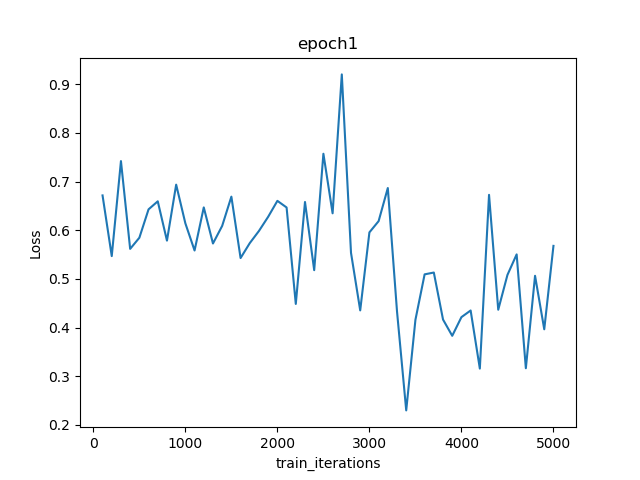
\includegraphics[width=10cm, height=7cm]{vgg16_bn_32_hybrid.png}

Figure: Hybrid VGG-16 with batchsize = 32

\subsection{Tuning Batch Size and Learning Rates}
From the previous experiments we noticed that different batch sizes in the training phase might give varying performance; e.g.  the smaller batch size of 8 took longer to train and performed considerably lower than larger batch sizes such as 16, 32 and 64. Moreover, we notice that larger mini-batches may tolerate higher learning rate without having gradient problems and thus speed up training. 

we soon noticed that when batch size exceeds the TitanX GPU on Gypsum would encounter memory error. And smaller batch sizes were already shown to have weaker performances and running time. So we conducted the following experiments with batchsize of 32 and 64 - and with each we tried learning rate of 1e-3, 1e-4, and 1e-5. 

The results are summarized in the table at section 5.7.


\subsection{Multiple Covariates}
A few more adjustments had to be made in order for our hybrid model to take multiple covariates at the same time. Now our structured covariates become a matrix $\mathbf{Cov}$ of shape (batchsize, num\_covariates), where every row of this matrix is an array of covariates. Picking `smiling', `high cheekbone' and `young' as our attributes, we have to internally loop over the 3 covariates to compute the kernel. 

The l-th kernel is computed from the scalar product between each initialized weight matrix and the scalar covariate value $S_{li}$ (0 or 1)
$$K_l = W_0 + W_1 \cdot S_{l1} + W_2 \cdot S_{l2} + W_3 \cdot S_{l3}...$$

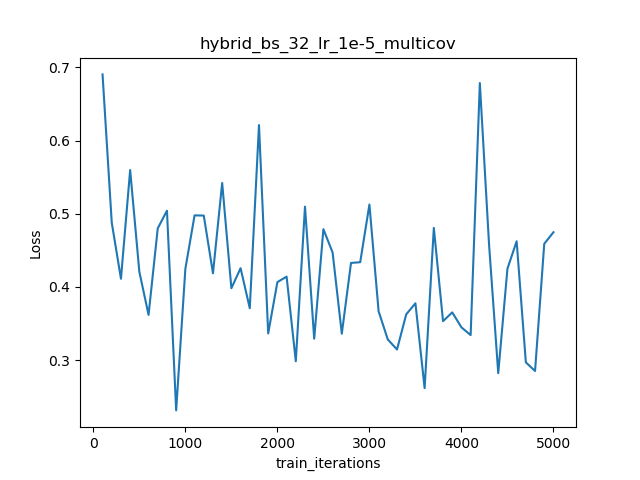
\includegraphics[width=10cm, height=7cm]{hybrid_bs_32_lr_1e-5_multicov.png}

Figure: Hybrid VGG16 with three covariates

\subsection{Relocating the Hybrid Layers}

Following the discussed in section 3, we performed the respective experiments regarding moving the hybrid layers to the later part of the VGG network. In a more detailed description, we inspected the source code of the VGG network, and noticed that all of the feature extracting layers (13 blocks of convolutional layers followed by non-linearity activation and batch normalization) are contained together. Therefore it is relatively easy to take out any of the convolutional layers and replace it with our hybrid layer. 

we attempted to replace the second, third and the last (13th) convolutional layer with hybrid\_Conv2d, but for some reason the model experienced an unknown error when the hybrid layer was placed at the second block. We ended up obtaining error-free outputs from the other two experiments and the results are presented below.



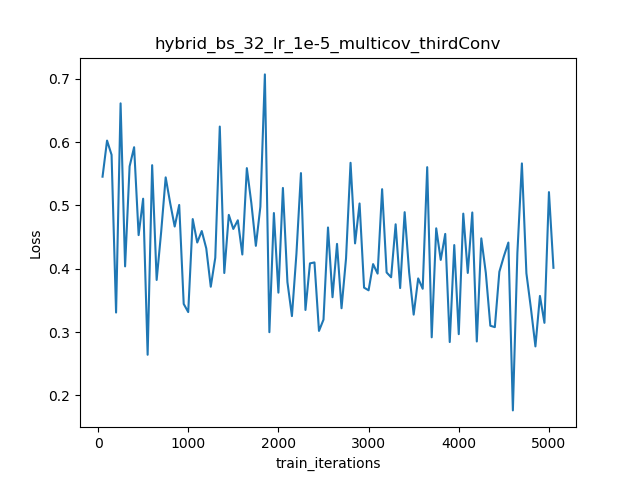
\includegraphics[width=10cm, height=7cm]{hybrid_bs_32_lr_1e-5_multicov_thirdConv.png}

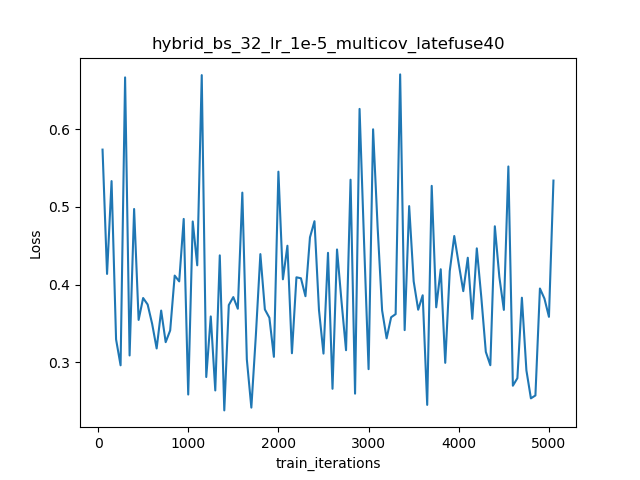
\includegraphics[width=10cm, height=7cm]{hybrid_bs_32_lr_1e-5_multicov_latefuse40.png}

Figure: Loss curve for hybrid layer replacing the 3rd and the last convolutional layer

\subsection{Results and Evaluation}
Here we summarize the results across all the significant experiments that we conducted into a table and we will discuss how the model performances changed over different settings. 

As we see from the summary, the baseline model performs under 0.80 accuracy when the batch size is smaller than 32. With one structured covariate (we choosed gender at the time), the accuracy was able to reach 0.80-0.81 with a tuned learning rate. We chose to run the rest of the experiments with the tuned batchsize and learning rate. We only moved the position of the hybrid layer when we had three covariates, and the resulting accuracy was consistently above 0.81. 

The best performing configuration was replacing the last convolutional layer in VGG-16 with our hybrid layer, running on batchsize=32 and learning rate of 1e-5, having three covariates (smiling, young, and high cheekbone) and using the Adam optimizer and binary cross entropy loss. We trained on the entire training set which had over 5000 iterations and the evaluated on the entire validation set. F1 macro score and binary accuracy were very close, both around 0.821. 


    \begin{center}
        \begin{tabular}{|c|c|c|c|c|} \hline
        model & batch\_size & learning\_rate & experiment type & Accuracy  \\ 
                           \hline
        Baseline           & 8           & 1e-03       & baseline                 & 0.79217              \\
        Baseline           & 16          & 1e-03       & baseline                 & 0.79604              \\
        Baseline           & 32          & 1e-03       & baseline                 & 0.80661              \\
        Baseline           & 64          & 1e-03       & baseline                 & 0.80505              \\
        Hybrid\_one\_cov   & 16          & 1e-03       & varying\_batch\_size     & 0.78285              \\
        Hybrid\_one\_cov   & 32          & 1e-03       & varying\_batch\_size     & 0.78804              \\
        Hybrid\_one\_cov   & 64          & 1e-03       & varying\_batch\_size     & 0.79946              \\
        Hybrid\_one\_cov   & 32          & 1e-04       & varying\_lr              & 0.81199              \\
        Hybrid\_one\_cov   & 32          & 1e-05       & varying\_lr              & 0.81345              \\
        Hybrid\_one\_cov   & 64          & 1e-04       & varying\_lr              & 0.81018              \\
        Hybrid\_one\_cov   & 64          & 1e-05       & varying\_lr              & 0.80414              \\
        Hybrid\_one\_cov   & 64          & 1e-06       & varying\_lr              & 0.76458              \\
        Hybrid\_three\_cov & 32          & 1e-05       & multiple\_covariates     & 0.81281              \\
        Hyrbid\_1st\_conv  & 32          & 1e-05       & varying\_layer\_position & 0.81269                     \\
        Hyrbrid\_3rd\_conv & 32          & 1e-05       & varying\_layer\_position & 0.81053                     \\
        Hybrid\_last\_conv & 32          & 1e-05       & varying\_layer\_position & \textbf{0.82136}        \\
        \hline
        \end{tabular}
    \end{center}


\section{Conclusion}
In this paper we presented how incorporating structured covariates can bring performance boost for deep learning models in classifying visual data. We tested our hypothesis on the CelebA dataset which contains more than 100,000 human faces and a rich array of facial attribute annotations. By incorporating multiple other facial attributes into the convolutional layers of our network, we were able to get better prediction results on certain target attributes such as `attractiveness'. We first established a baseline model using VGG-16 network and performed binary classification on CelebA, trained on 162,770 instances and validated our results on a separate validation set of 19,867 images. We evaluated our model using macro F1 score and binary accuracy, and the initial baseline performance metric is consistently at 0.78-0.79. In detailed documentation, we then developed a hybrid convolutional layer and substituted the \textit{Conv2d} layer in VGG with it. At the earlier stage we only allowed one structured covariate to pass through the network along with its corresponding image at each iteration, but later we enabled the hybrid network to take an array of multiple covariates along with each image. We then conducted experiments to find the best fitting hyperparameters such as the size of mini-batches and the learning rate. For each of the experiments we plotted the loss curves and saved the best-performing model checkpoint, in addition to recording the evaluation metrics. We also explored the effects of replacing the later convolutional layers with the hybrid layer, in attempt to fuse the structured information with higher-level image features. We found that although overall did not have a very significant difference, placing the hybrid layers at the end of the deep network occasionally had stronger performance than their counterparts in the early layers. 

\subsection{Discussions and Future Work}
This thesis project mainly investigated the creation of hybrid convolution with structured covariate and a practical implementation of Shortfused hybrid convolutional neural network. We used a VGG network for our experiments, but from the literature we have reviewed in previous sections, we observe that the InceptionNet-V3 is known to have better performance and holds the current State-of-the-Art in the CelebA facial attribute prediction task [reference]. However, since the convolutional operation in different network architectures remain very similar to each other, we believe that it'd be relatively easy to apply our hybrid mechanism to other networks as well. Besides, keep in mind that our real focus of this shortfuse technique is not merely to improve performance on facial attribute prediction, but rather on feature extraction for neuroimages such as brain MRIs, so as long as we know that the structured covariates do improve our Convolutional Networks, we have reasons to believe that this approach will have positive benefits for our future work.  


This idea of bringing structured information into CNNs originated from our interest in brain scans and more specifically Alzheimer's detection/automatic diagnosis. Despite the 3-dimensional, volumetric nature of MRI data, we believe that it will not take too much effort to corporate my hybrid layers into the 3D convolutional network we obtain in the lab that is specialized in processing MRI images. 



\section{References}









\end{document}